\section{Backup modello di Ising 2D}

%----------------------------------------%
%		       Prima slide	     	     %
%	Osservabili per reticolo 100 x 100   %
%----------------------------------------%
\begin{frame}
    \frametitle{Osservabili per reticolo $100 \times 100$}
    \framesubtitle{}

    \centering
    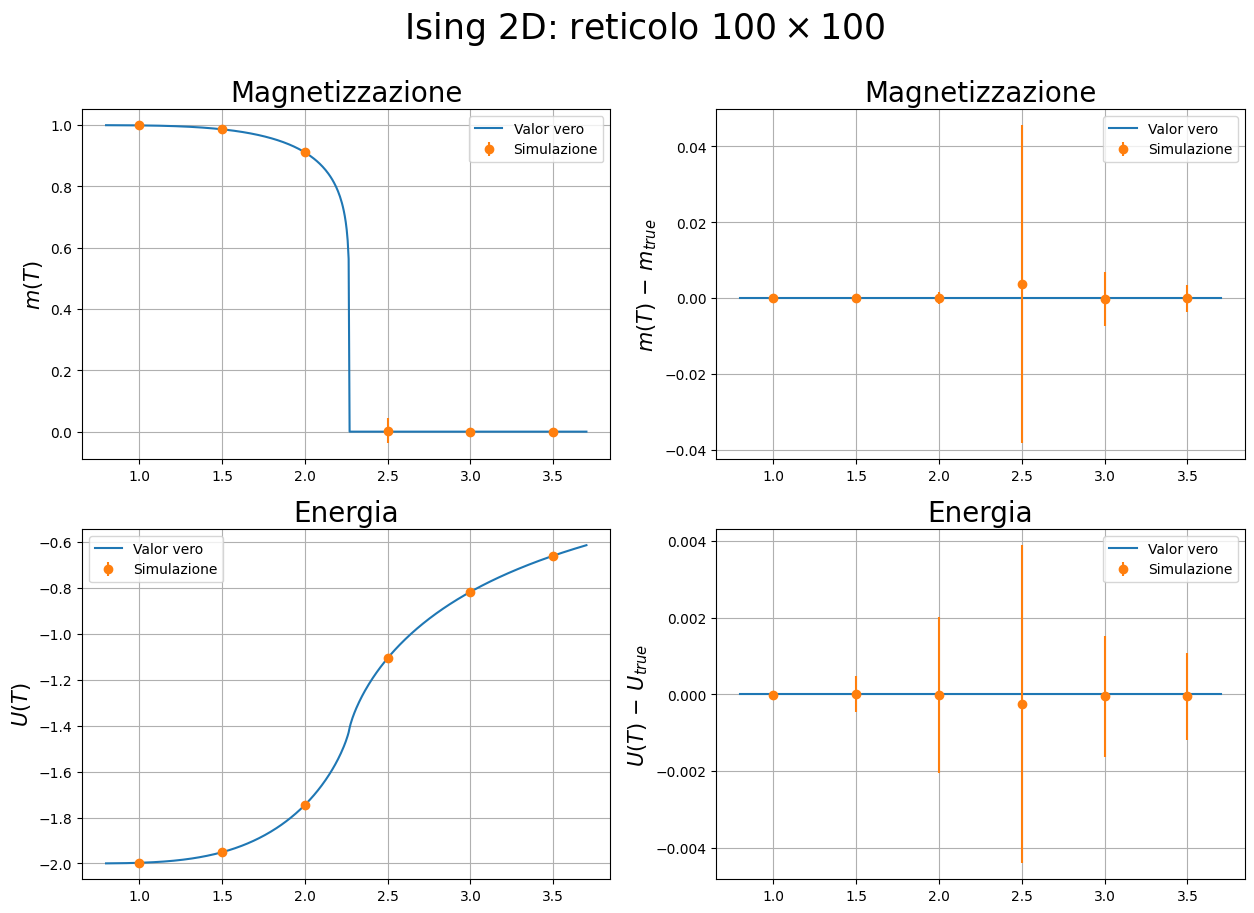
\includegraphics[width=0.65\textwidth]{Immagini/backupIsing2D/obs_100.png}

\end{frame}



%----------------------------------------%
%		      Seconda slide	     	     %
%	Osservabili per reticolo 100 x 100   %
%----------------------------------------%
\begin{frame}
    \frametitle{Osservabili per reticolo $200 \times 200$}
    \framesubtitle{}

    \centering
    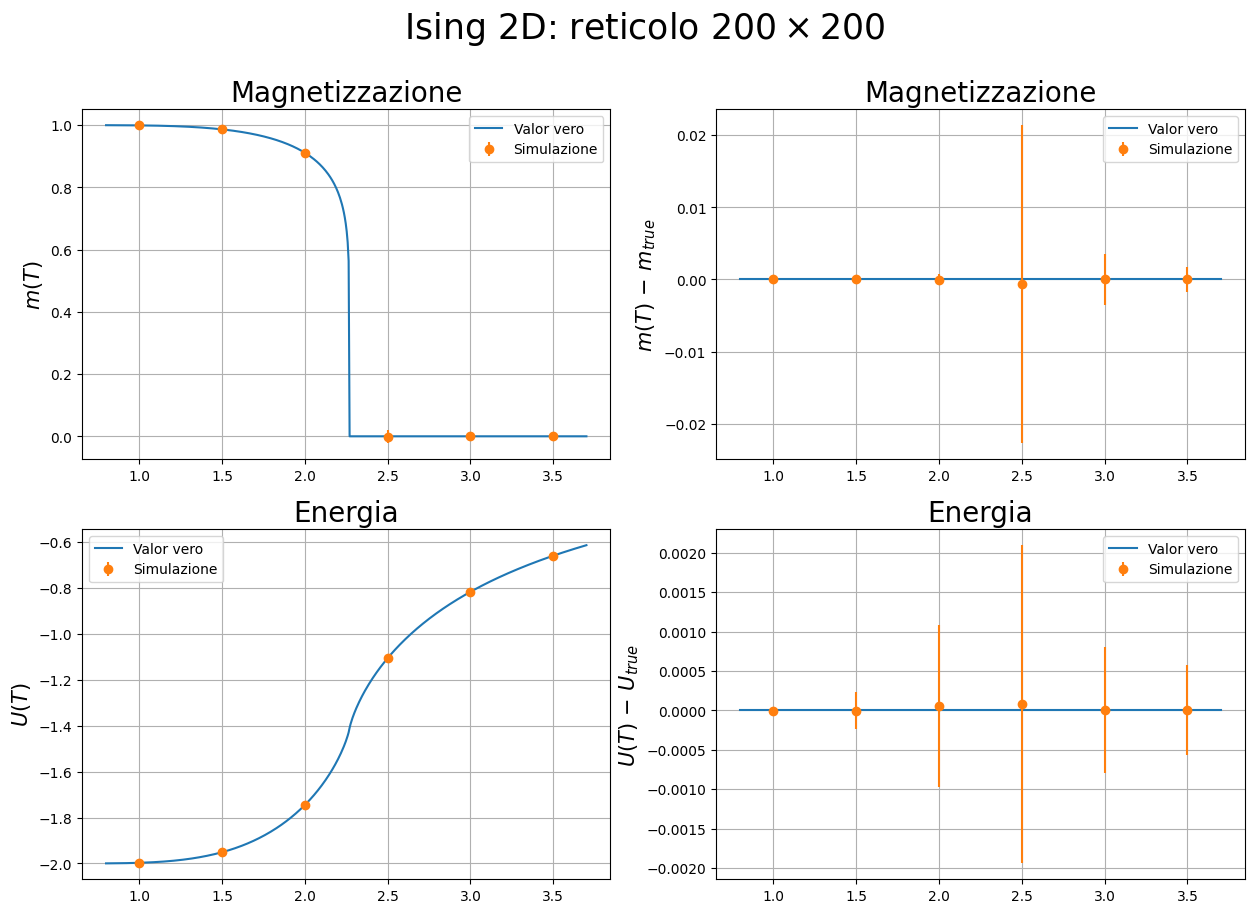
\includegraphics[width=0.65\textwidth]{Immagini/backupIsing2D/obs_200.png}

\end{frame}



%----------------------------------------%
%		       Terza slide	     	     %
%	Osservabili per reticolo 300 x 300   %
%----------------------------------------%
\begin{frame}
    \frametitle{Osservabili per reticolo $300 \times 300$}
    \framesubtitle{}

    \centering
    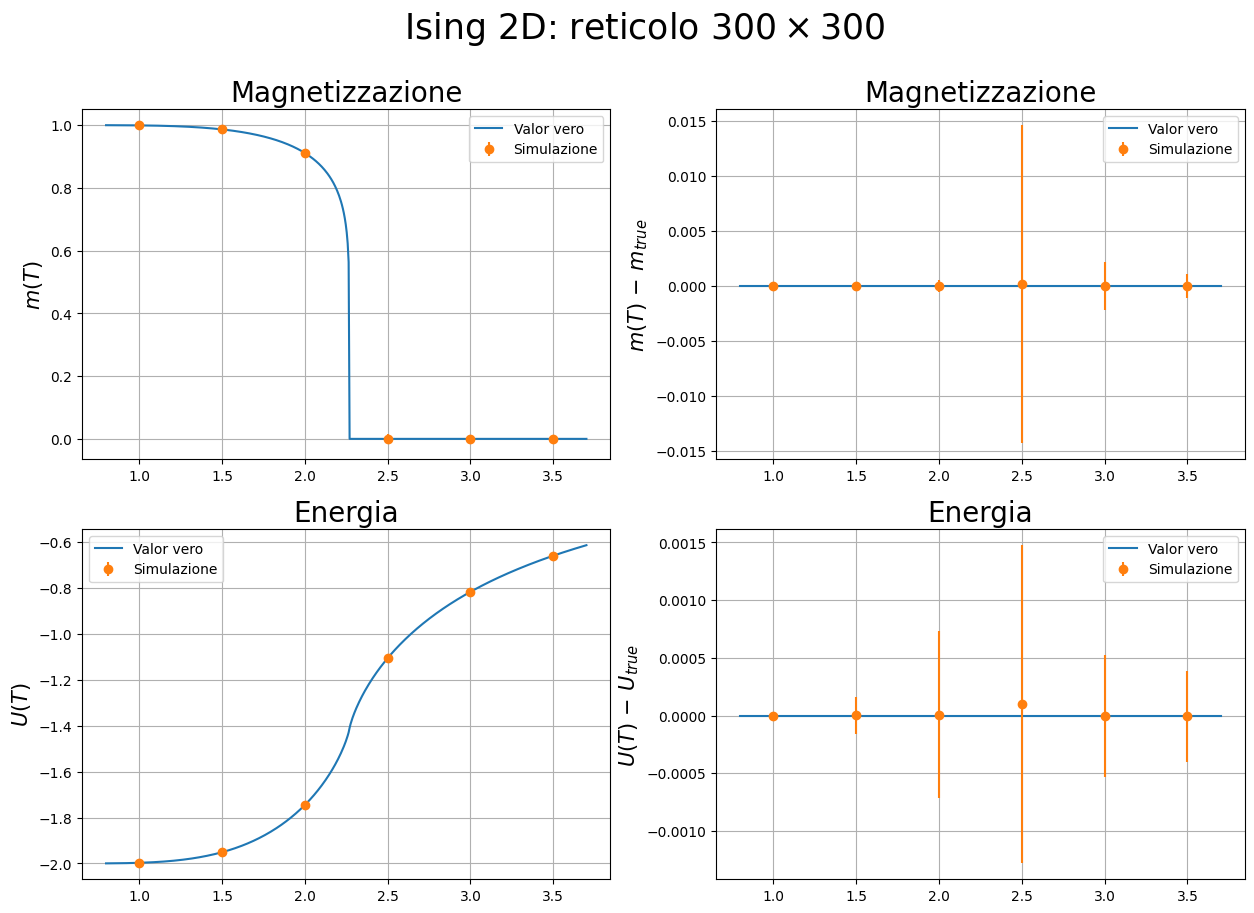
\includegraphics[width=0.65\textwidth]{Immagini/backupIsing2D/obs_300.png}

\end{frame}



%----------------------------------------%
%		       Quarta slide	     	     %
%	Osservabili per reticolo 400 x 400   %
%----------------------------------------%
\begin{frame}
    \frametitle{Osservabili per reticolo $400 \times 400$}
    \framesubtitle{}

    \centering
    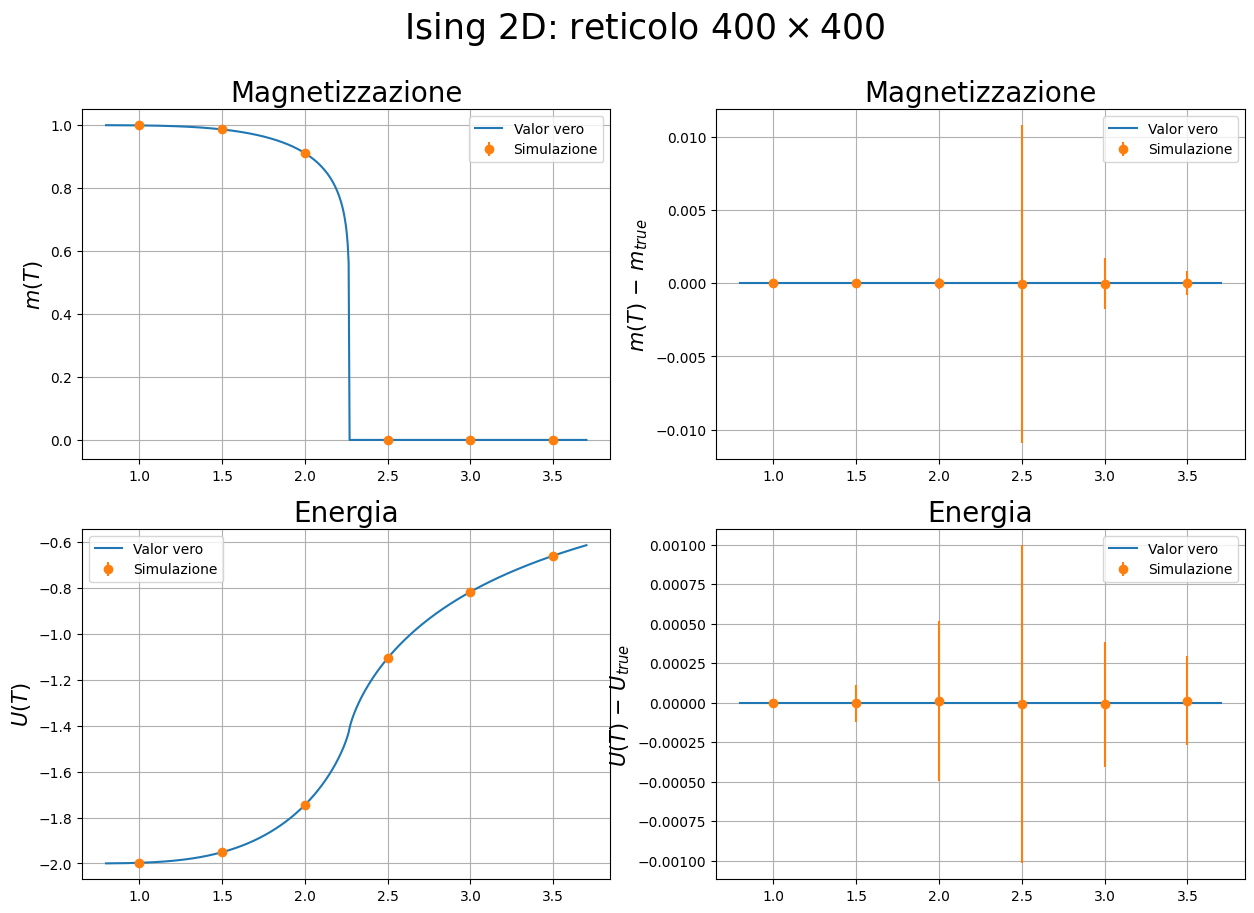
\includegraphics[width=0.65\textwidth]{Immagini/backupIsing2D/obs_400.png}

\end{frame}



%----------------------------------------%
%		       Quinta slide	     	     %
%	Osservabili per reticolo 500 x 500   %
%----------------------------------------%
\begin{frame}
    \frametitle{Osservabili per reticolo $500 \times 500$}
    \framesubtitle{}

    \centering
    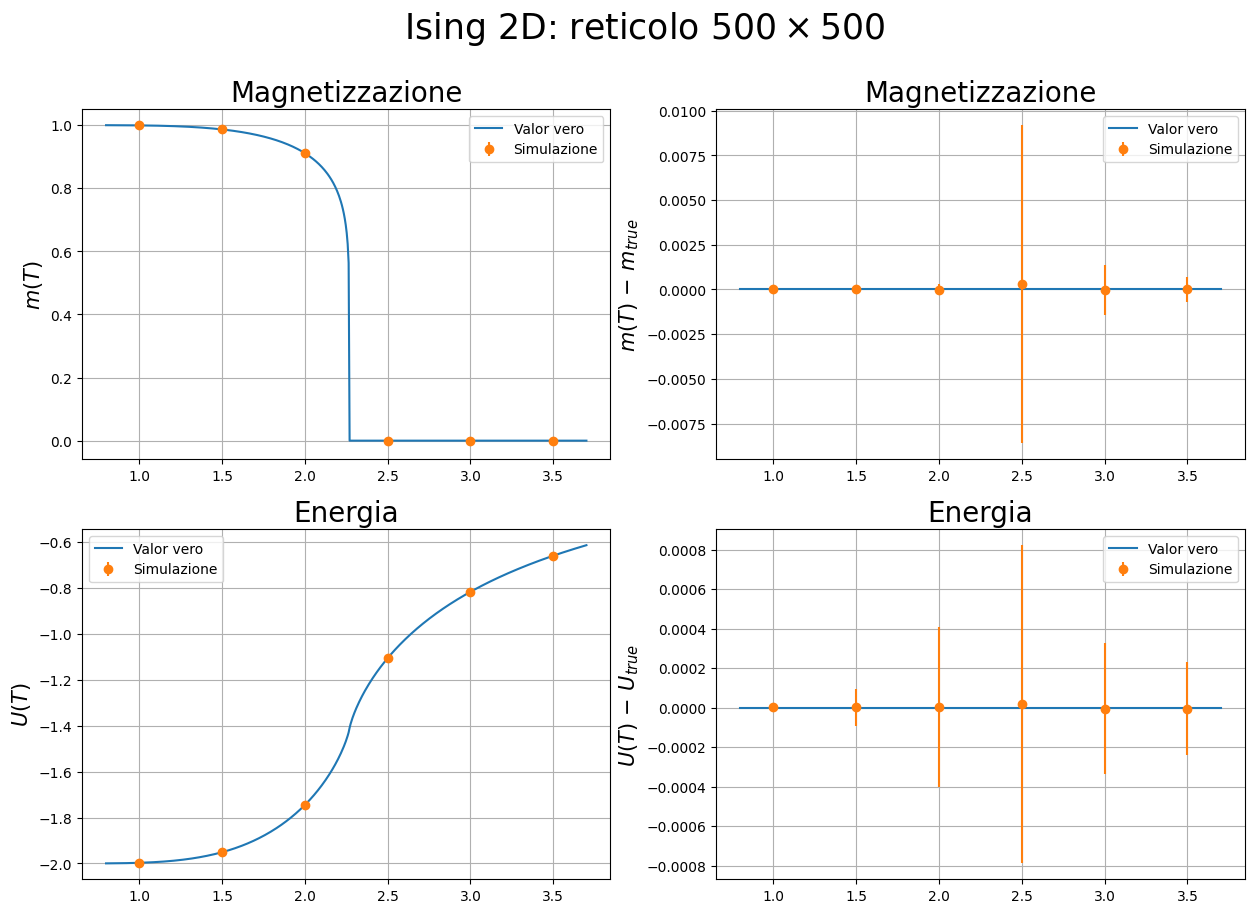
\includegraphics[width=0.65\textwidth]{Immagini/backupIsing2D/obs_500.png}

\end{frame}
